\section{Simulation Evidence on the Theoretical Mechanism}
\label{sec:simulation_mechanism}

This section uses simulations as a bridge between the task-level model and the panel specification. The simulations are not used as causal evidence. Instead, they clarify the model's mechanics and show when the empirical specification recovers the structural effect embedded in the data-generating process.

\subsection{Task Exposure and Entry Thresholds}

The first simulation generates task-level human productivity $h_c(z)$ and ChatGPT productivity $a_c(z)$ for each programming language. For each language, we compute the automated-task set $\mathcal{Z}^{auto}_c=\{z:a_c(z)>h_c(z)\}$, the automated-task share $\tau_c$, the average relative saving $\rho_c$, and the exposure index $\theta_c=\tau_c\rho_c$. Figure~\ref{fig:sim_language_exposure} reports the simulated exposure measures by language.

\begin{figure}[!htbp]
\centering
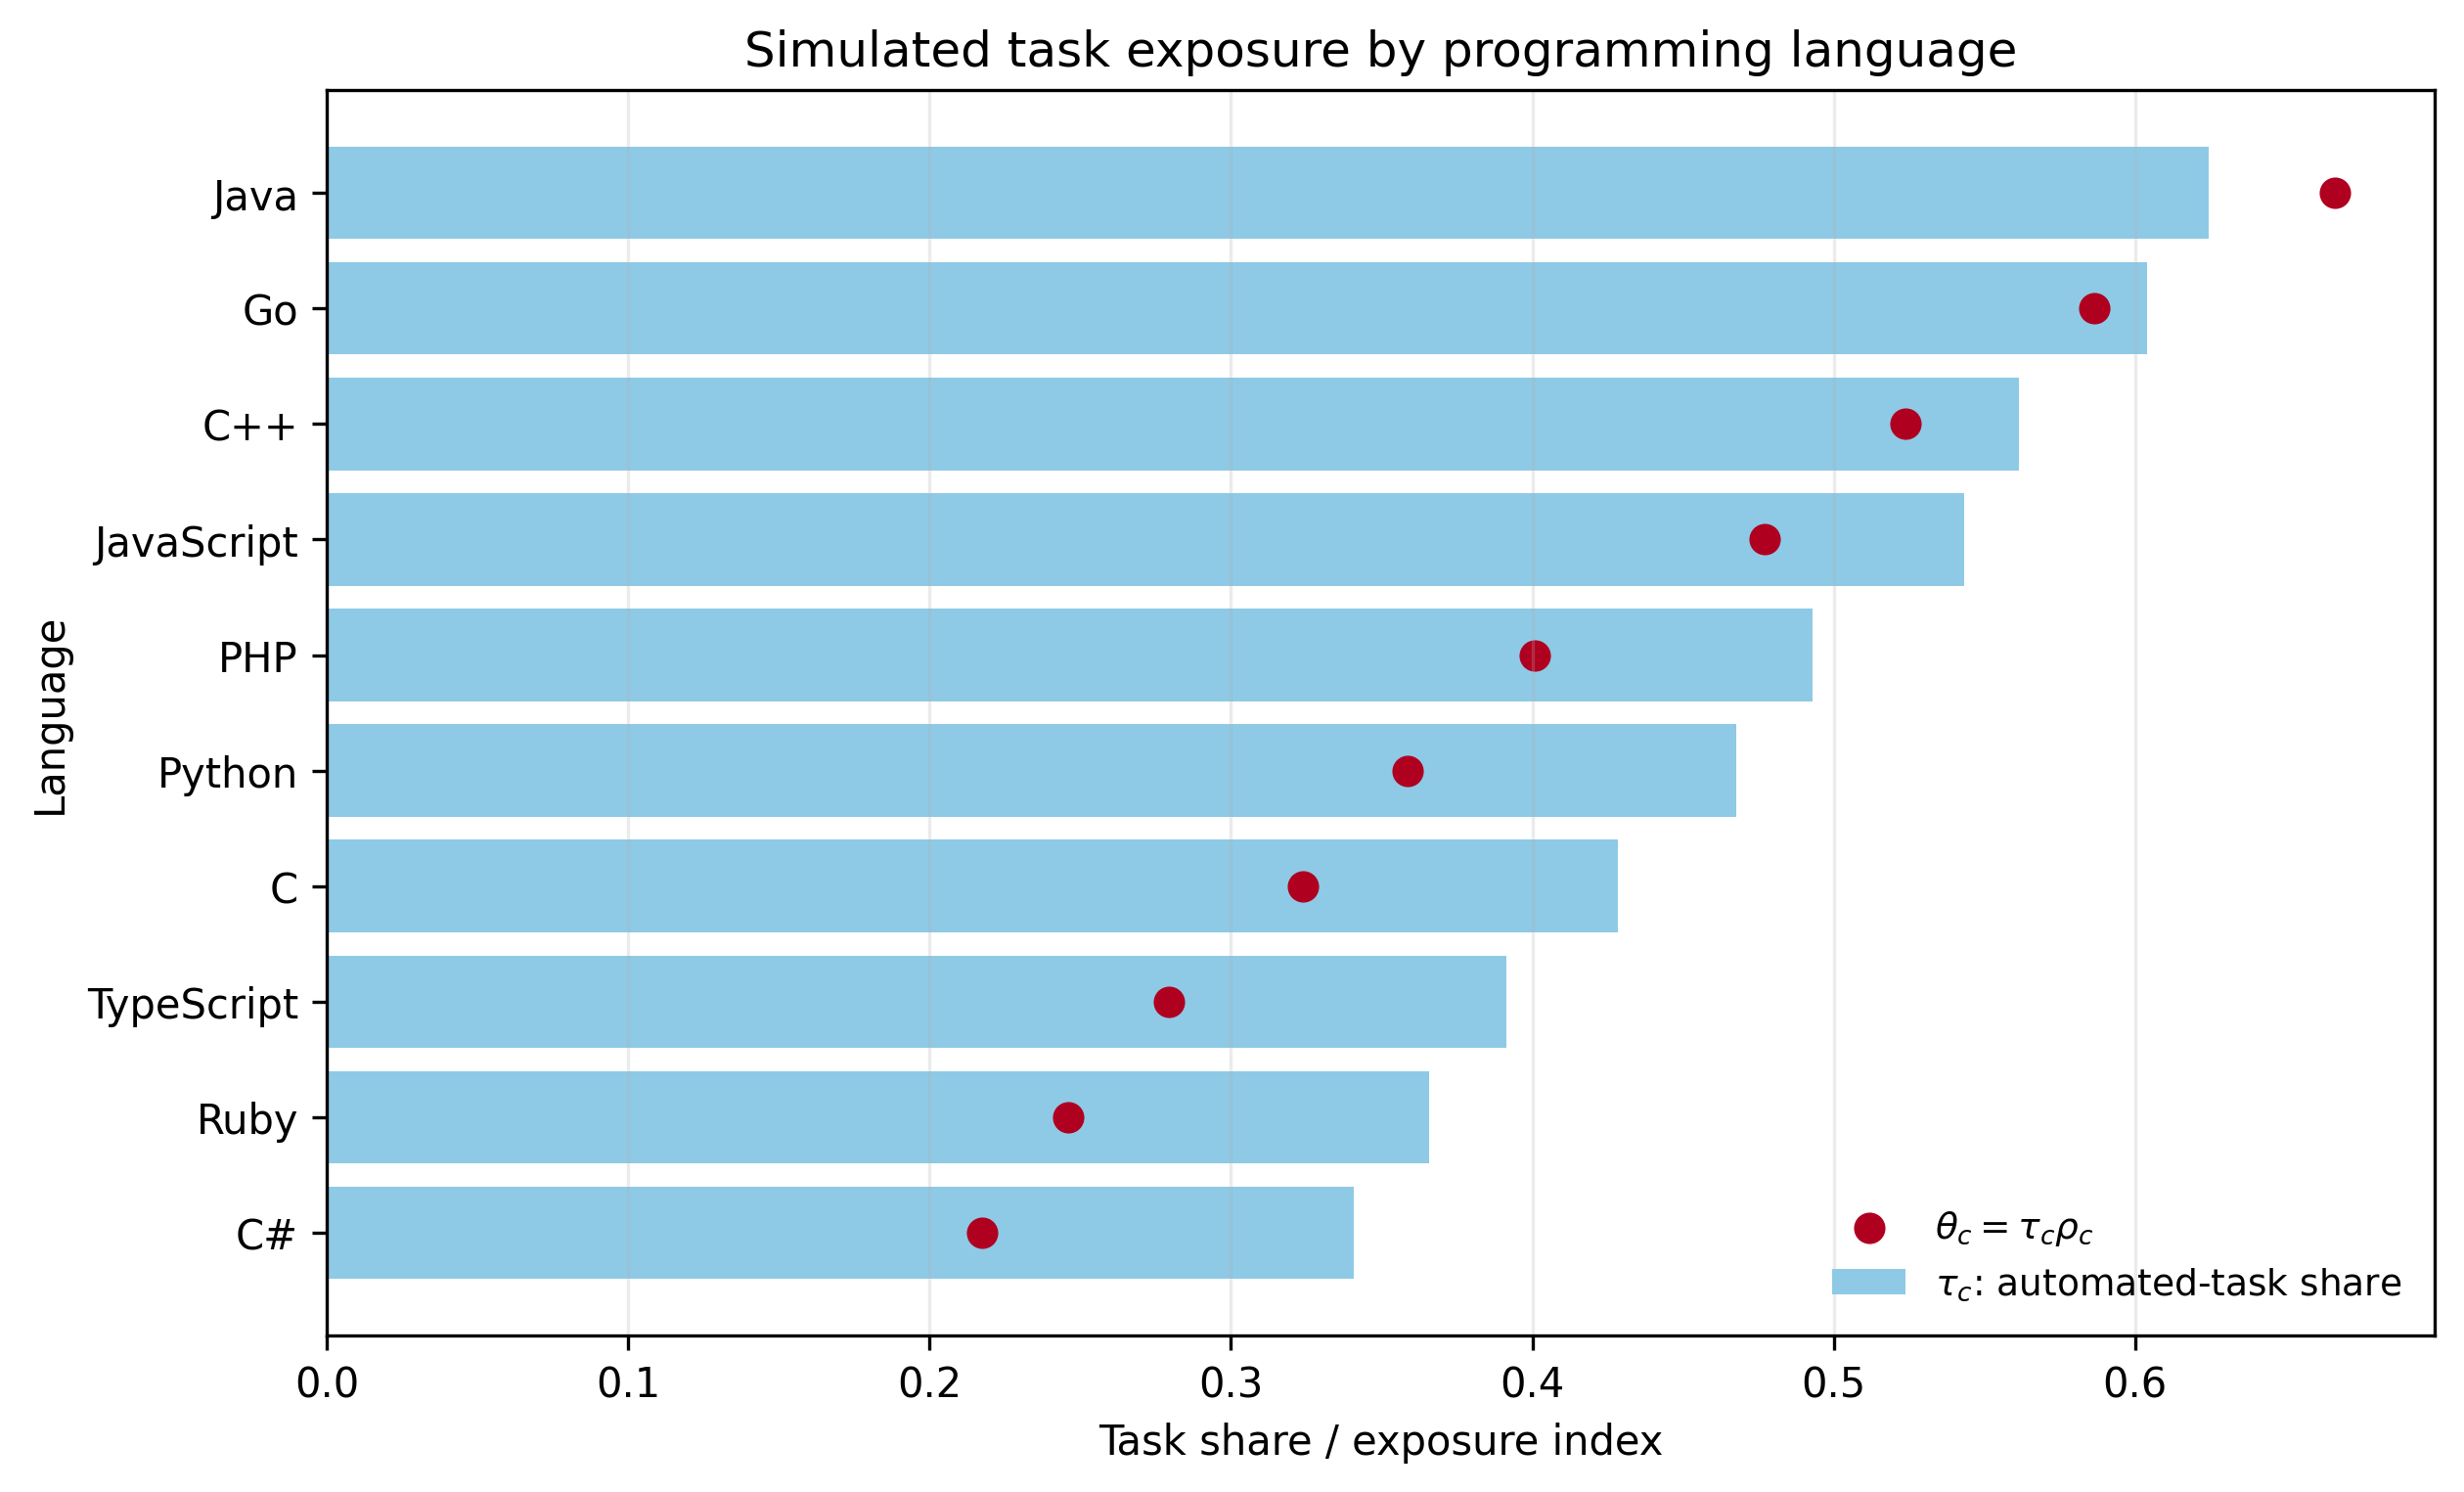
\includegraphics[width=0.82\linewidth]{output/figures/simulations/sim_language_exposure.png}
\caption{Simulated task exposure by programming language}
\label{fig:sim_language_exposure}
\end{figure}

The second simulation maps the productivity gain into the entry margin. The model implies that access to AI lowers the entry threshold from $\eta_c^*(0)$ to $\eta_c^*(1)=\eta_c^*(0)-\tau_c\rho_c$. Figure~\ref{fig:sim_threshold_entry} illustrates the mass of marginal entrants located between the old and new thresholds.

\begin{figure}[!htbp]
\centering
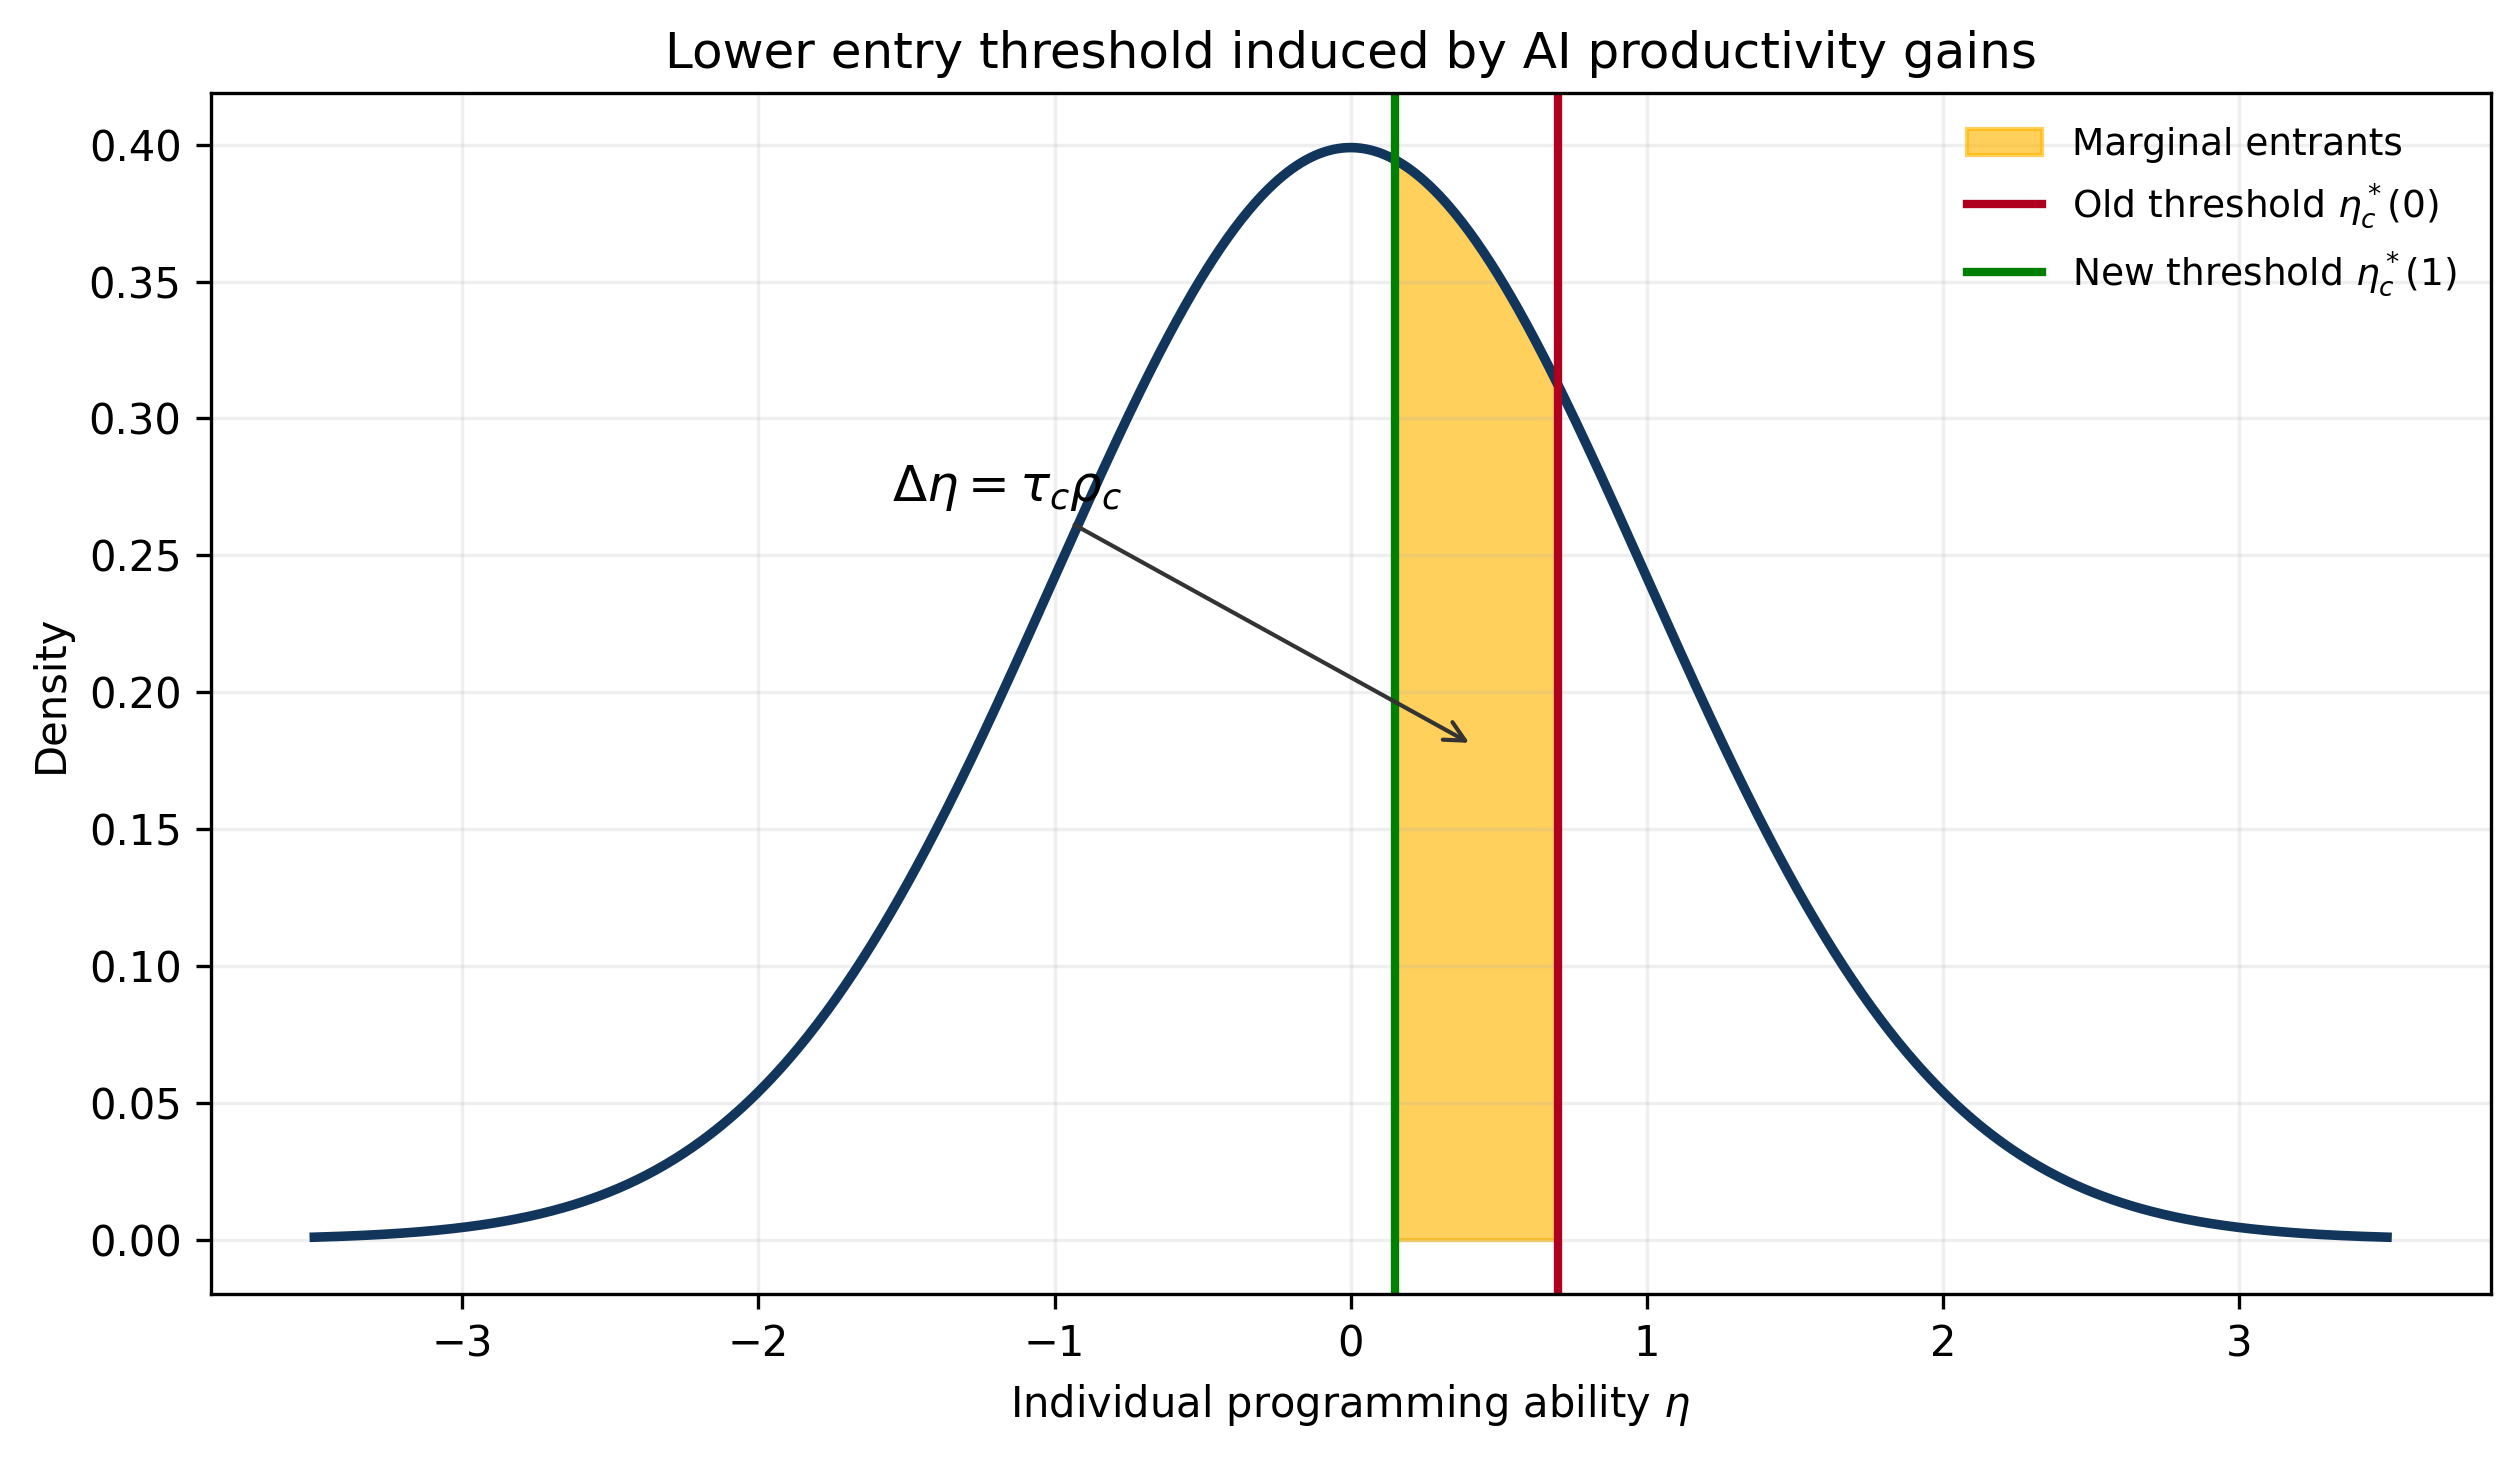
\includegraphics[width=0.78\linewidth]{output/figures/simulations/sim_threshold_entry.png}
\caption{Lower entry threshold induced by AI productivity gains}
\label{fig:sim_threshold_entry}
\end{figure}

Combining language exposure with country-level absorption produces the prediction $\Delta Y_{ic}\approx \phi_i\theta_c$. Figure~\ref{fig:sim_theta_entry_relationship} shows that predicted entry is increasing in language exposure, with steeper responses in high-absorption countries.

\begin{figure}[!htbp]
\centering
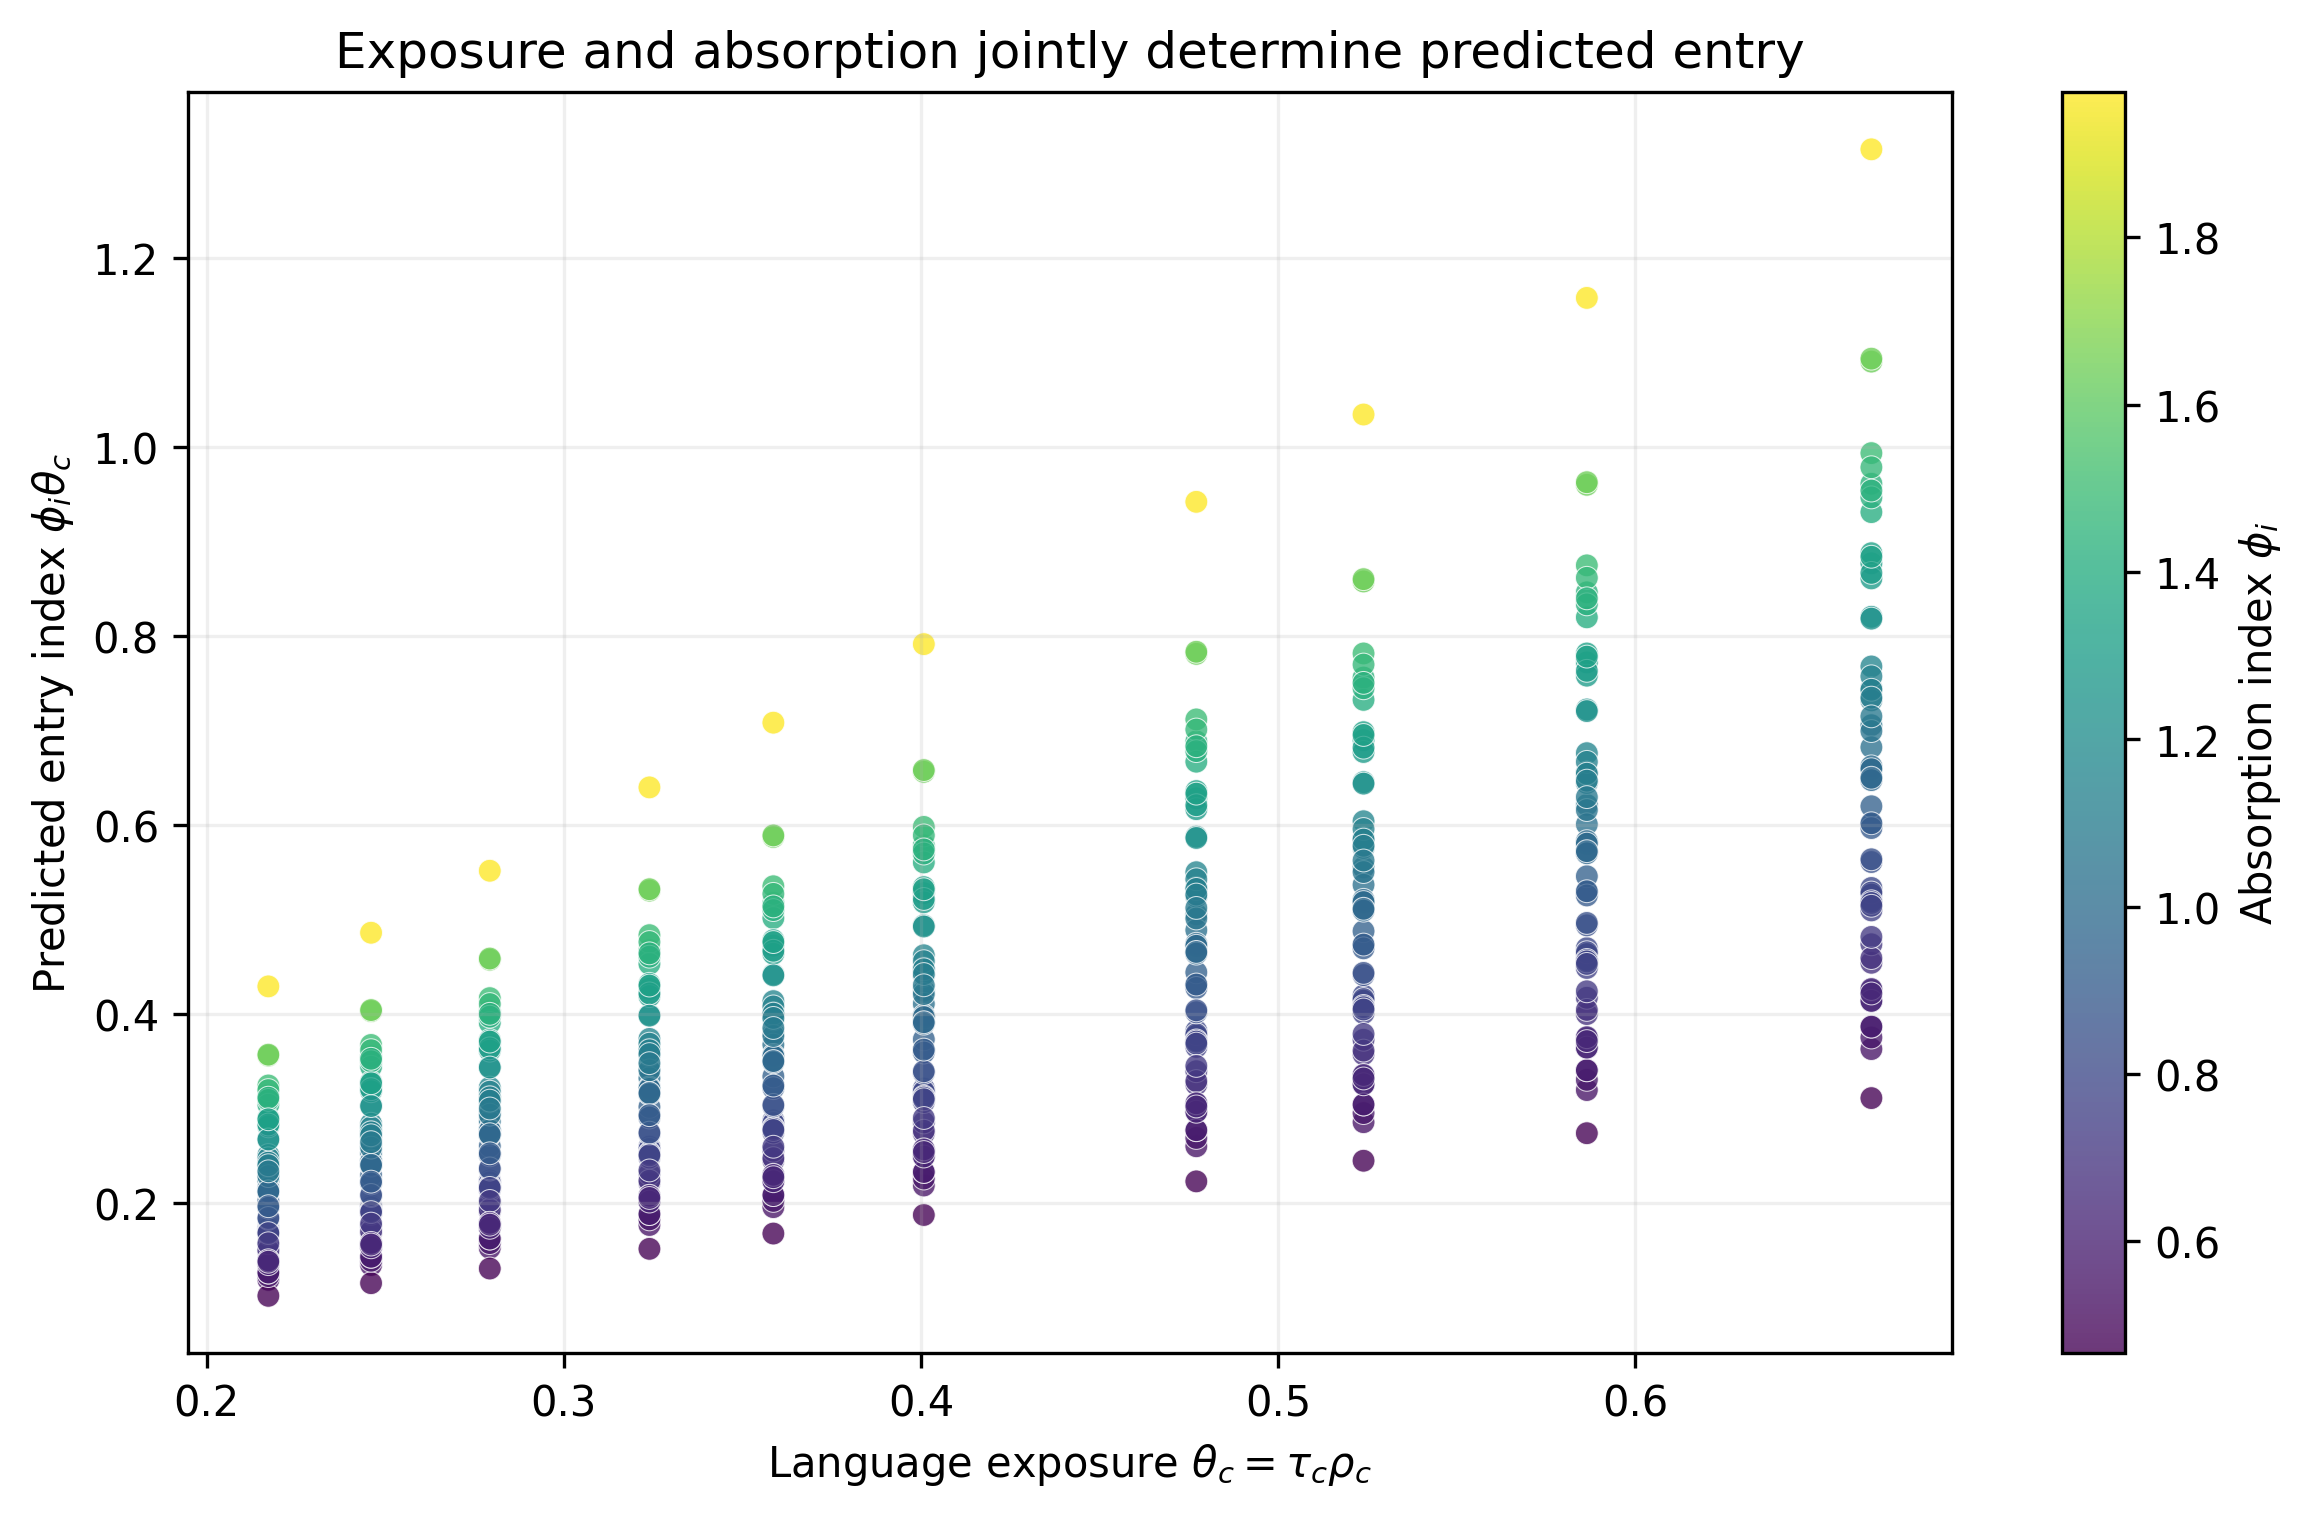
\includegraphics[width=0.78\linewidth]{output/figures/simulations/sim_theta_entry_relationship.png}
\caption{Exposure and absorption jointly determine predicted entry}
\label{fig:sim_theta_entry_relationship}
\end{figure}

\subsection{Sensitivity to the Covariance Assumption}

The simplified model imposes $\operatorname{Cov}_{\mathcal{Z}^{auto}_c}(h_c,s_c)=0$, which yields $\Delta y_{jc}=\tau_c\rho_c$ after normalizing $\bar h_c=1$. The exact normalized gain is
\[
\Delta y_{jc}=\tau_c\left[\rho_c+\operatorname{Cov}_{\mathcal{Z}^{auto}_c}(h_c,s_c)\right].
\]
Figure~\ref{fig:sim_covariance_sensitivity} varies the correlation between human productivity and AI relative savings. The simplified exposure index closely tracks the exact gain near zero covariance, but it understates or overstates the gain when the covariance term becomes economically meaningful.

\begin{figure}[!htbp]
\centering
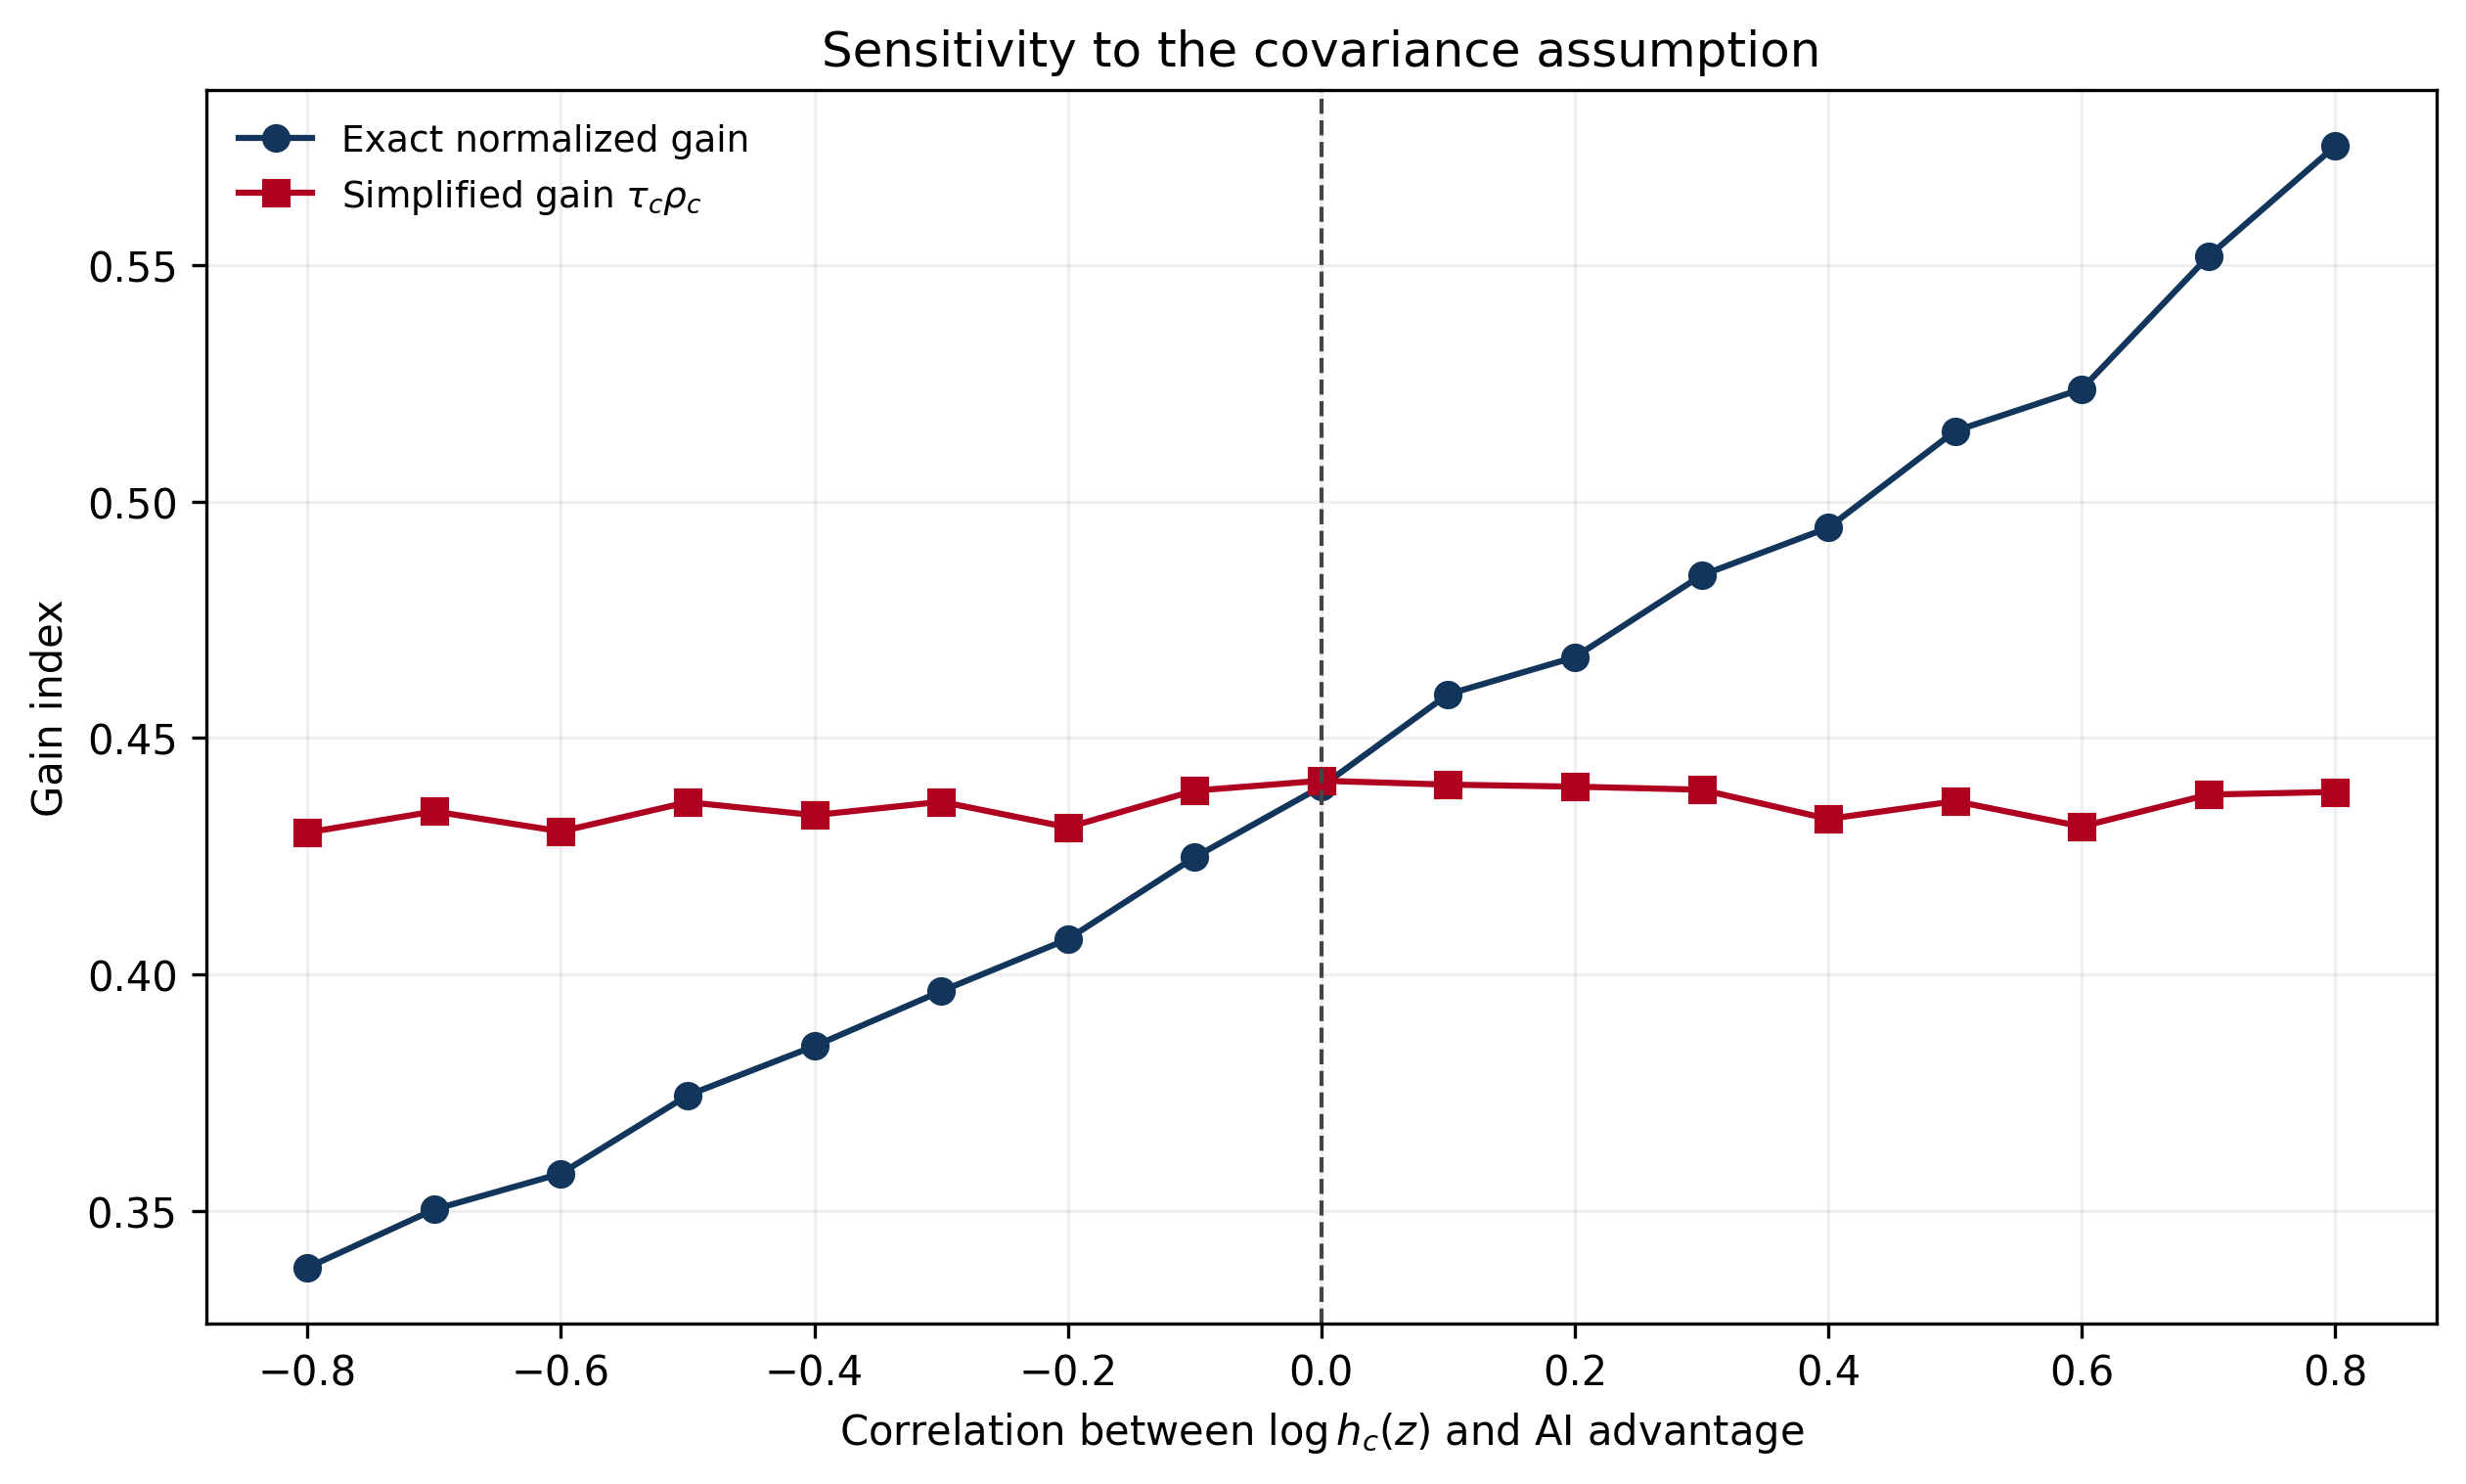
\includegraphics[width=0.78\linewidth]{output/figures/simulations/sim_covariance_sensitivity.png}
\caption{Sensitivity to the covariance assumption}
\label{fig:sim_covariance_sensitivity}
\end{figure}

\subsection{Monte Carlo Recovery of the Panel Estimator}

The final simulation generates panel data from
\[
Y_{ict}=\alpha_i+\beta_t+\delta_c+\theta_c\phi_i A_{it}+\eta_{ict},
\]
and estimates the same fixed-effects specification used in the empirical design. Table~\ref{tab:sim_monte_carlo} reports 500 Monte Carlo replications. Under exogenous treatment assignment, the estimator is centered around the true effect. When simulated shocks violate the identifying assumptions, the estimated coefficient becomes biased, which clarifies the role of the event-study, placebo, and robustness exercises in the empirical analysis.

\begin{table}[!htbp]
\centering
\caption{Monte Carlo recovery of the fixed-effects estimator}
\label{tab:sim_monte_carlo}
\small
\begin{tabular}{lllllll}
\toprule
Scenario & True beta & Mean estimate & Bias & RMSE & Mean SE & Coverage 95\% \\
\midrule
Exogenous treatment & 1.000 & 1.001 & 0.001 & 0.025 & 0.026 & 0.962 \\
Treated post-trend & 1.000 & 1.072 & 0.072 & 0.076 & 0.026 & 0.214 \\
Language-time shock & 1.000 & 1.019 & 0.019 & 0.032 & 0.026 & 0.894 \\
Country-language absorption & 1.000 & 1.118 & 0.118 & 0.121 & 0.026 & 0.010 \\
\bottomrule
\end{tabular}
\end{table}

